\documentclass[xcolor={dvipsnames}]{beamer}
\usepackage{mymathstyle}
\usepackage{paper_commands}
\usepackage{wrapfig}

\usetheme{metropolis}
\metroset{
    titleformat=smallcaps,
    progressbar=foot,
    % numbering=fraction,
    % background=dark,
    % block=fill,
    sectionpage=progressbar, %simple
}

% caption set up
\setbeamertemplate{caption}[default]
\setbeamertemplate{caption label}{}

\setbeamercolor{alerted text}{fg=RoyalBlue}

% \usepackage[T1]{fontenc}
% \usepackage{lmodern}

\usepackage[sfdefault]{FiraSans}

% \usefonttheme{default}
% \usefonttheme{professionalfonts}
% \usefonttheme{structureitalicserif}
% \usefonttheme{structuresmallcapsserif}
% \usefonttheme{structurebold}
% \usefonttheme{serif}

\usefonttheme[onlymath]{serif} % already in import of beamer

% \setbeamercolor{block title}{bg=blue!50, fg=white}
% \setbeamercolor{block body}{bg=blue!10, fg=black}


\title{Disentangling and Integrating Relational and Sensory Information in Transformer Architectures}
\author{\textit{Awni Altabaa, John Lafferty}}
% \date{\today}
\institute{Yale University \\
arXiv:2405.16727, ICML '25}

\begin{document}

\maketitle

% \AtBeginSection[]
% {
%   \begin{frame}
%     \frametitle{Table of Contents}
%     \tableofcontents[currentsection]
%   \end{frame}
% }

\section{Big Picture: Why should we care about ``relational reasoning''?}

\begin{frame}{The Fundamental Principles of Intelligence}
    \begin{itemize}
        \item \alert{\texttt{Hypothesis 0}:} Human \& animal intelligence can be explained by a few core principles (rather than an encyclopedic list of heuristics)
        % \item I.e., analogous to fundamental laws of physics
        \item \alert{Suggests the following goal:} Study \& uncover the inductive biases that humans \& animals exploit (to understand intelligence generally and inform design of AI)
        % \item Deep learning systems themselves exploit several key inductive biases that underly their empirical success
        % \item \alert{Goal of AI Research:} Uncover a core set of inductive biases for DL that enable data-efficient learning and reasoning over wide rang of tasks and modalities
        % % \item Principles alone not sufficient to predict behavior of complex systems (i.e., brains), 
        % \item \alert{\texttt{Hypothesis 1}:} Relational reasoning is one of these fundamental principles of intelligence
    \end{itemize}
\end{frame}

\begin{frame}{The Fundamental Principles of Intelligence}
    \begin{itemize}
        % \item \alert{\texttt{Hypothesis 0}:} Human \& animal intelligence can be explained by a few core principles (rather than an encyclopedic list of heuristics)
        % % \item I.e., analogous to fundamental laws of physics
        % \item \alert{Suggests the following goal:} Study \& uncover the inductive biases that humans \& animals exploit (to understand intelligence and inform design of AI)
        \item Deep learning systems themselves exploit several key inductive biases that underly their empirical success
        \item \alert{Goal of AI Research:} Uncover a core set of inductive biases for DL that enable data-efficient learning and reasoning over wide rang of tasks and modalities
        % \item Principles alone not sufficient to predict behavior of complex systems (i.e., brains), 
        \item \alert{\texttt{Hypothesis 1}:} Relational reasoning is one of these fundamental principles of intelligence
    \end{itemize}
\end{frame}


\begin{frame}{First: What is ``relational reasoning''?}
    \begin{itemize}
        \item Comparison
        \item Analogy
        \item Abstraction
    \end{itemize}
\end{frame}

\begin{frame}[standout]
    Let's walk through a couple simple illustrative examples of relational tasks
\end{frame}

\begin{frame}{Example: \textit{SET!} Card Game}
    % Relational reasoning: comes naturally to us humans; holds a special place in our minds / we have a preference for it; something we enjoy as a way to exercise our brains
    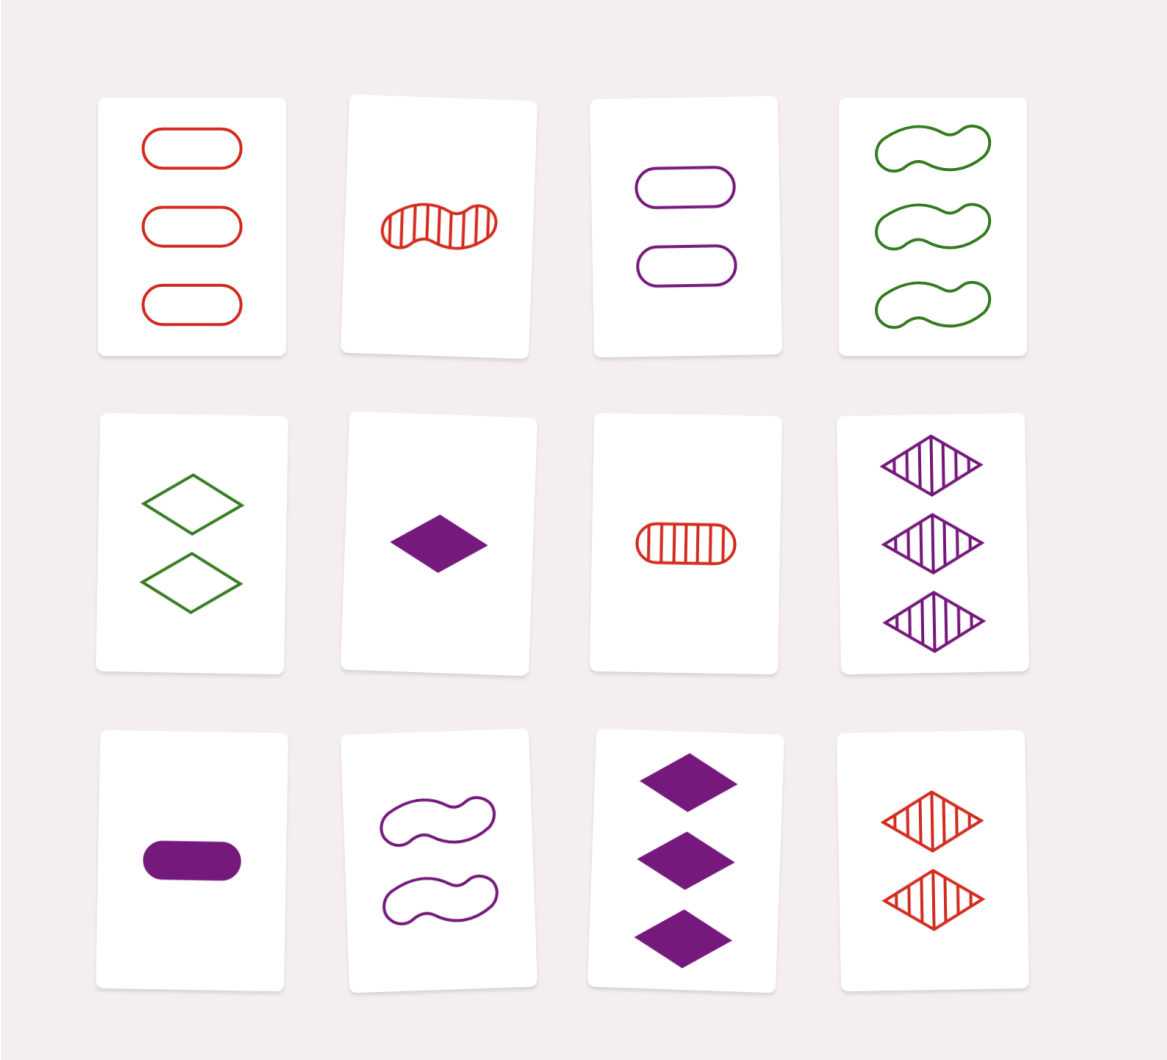
\includegraphics[width=0.8\linewidth]{figs/set_1.png}
\end{frame}

\begin{frame}{Example: \textit{SET!} Card Game}
    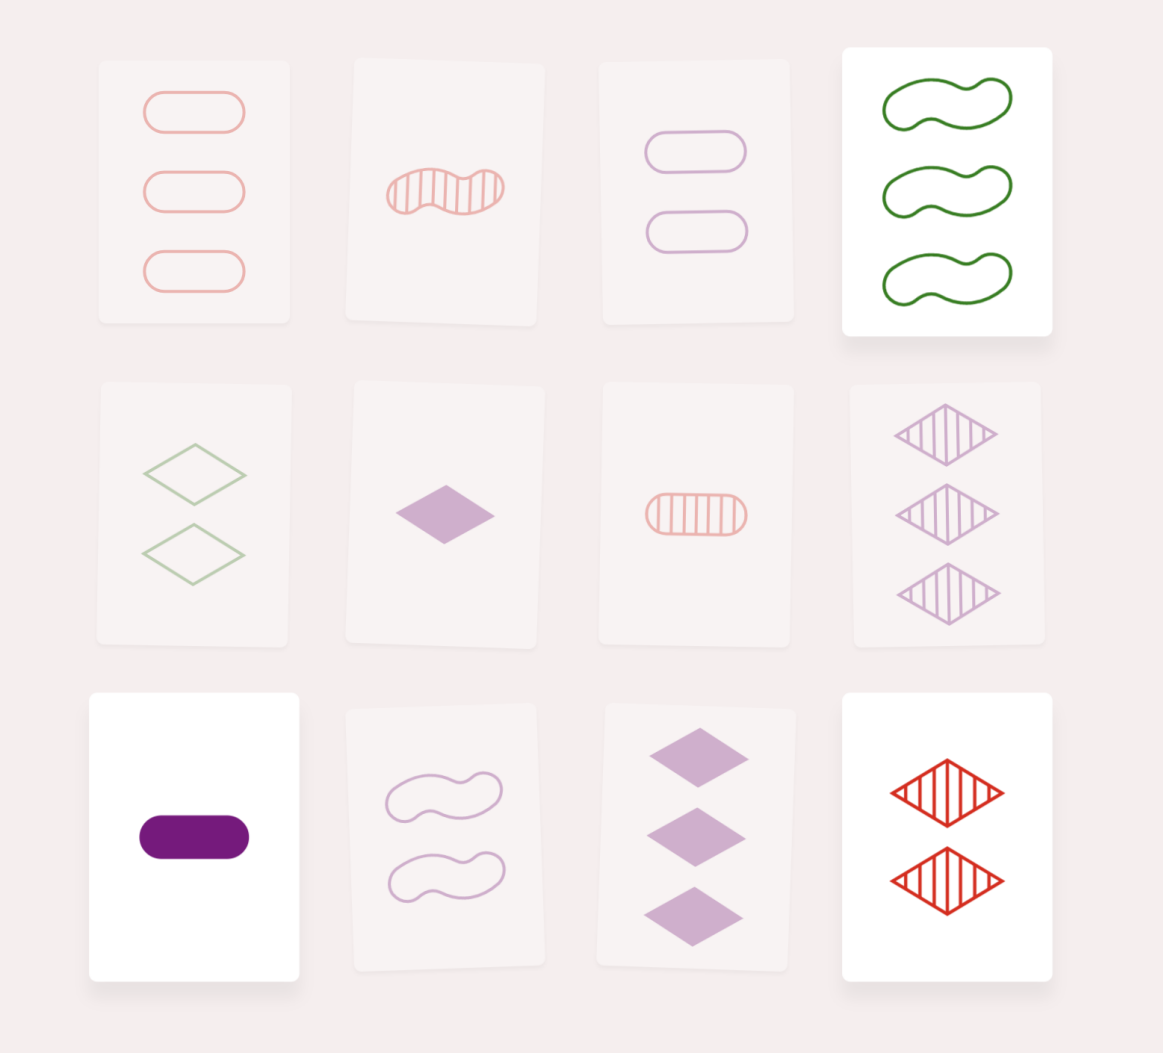
\includegraphics[width=0.8\linewidth]{figs/set_2.png}
\end{frame}

\begin{frame}{Example: Relational Games (Shanahan et al. 2020)}
    % \begin{wrapfig}{r}{0.75\linewidth}
    %     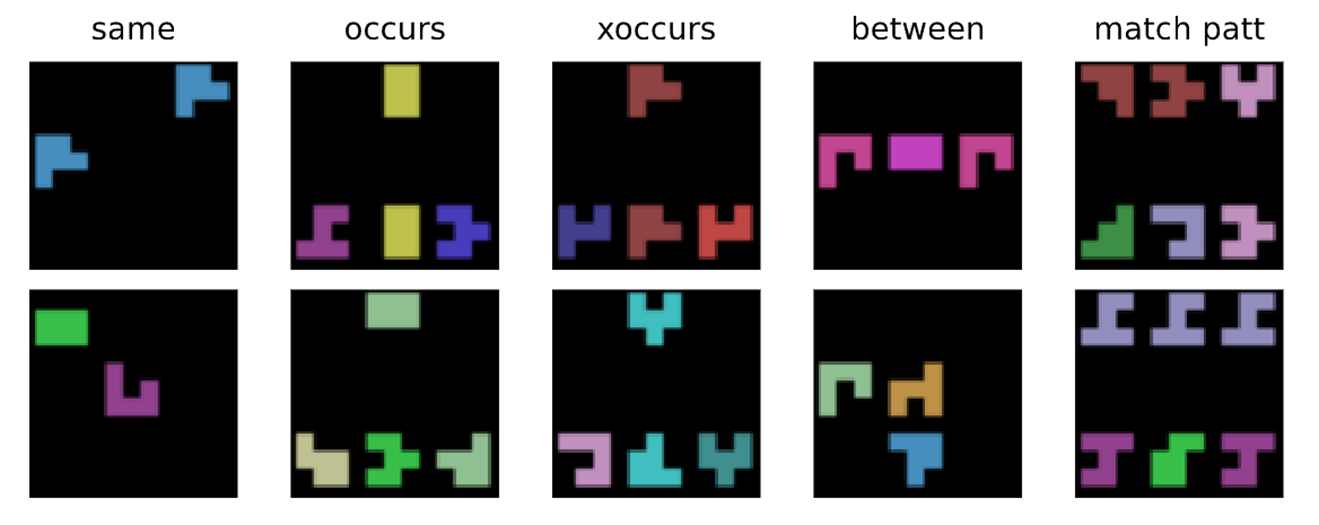
\includegraphics[width=\linewidth]{figs/relgames_example.png}
    %     \caption{Relational Games tasks from Shanahan et al. (2020)}
    % \end{wrapfig}
    \begin{figure}
        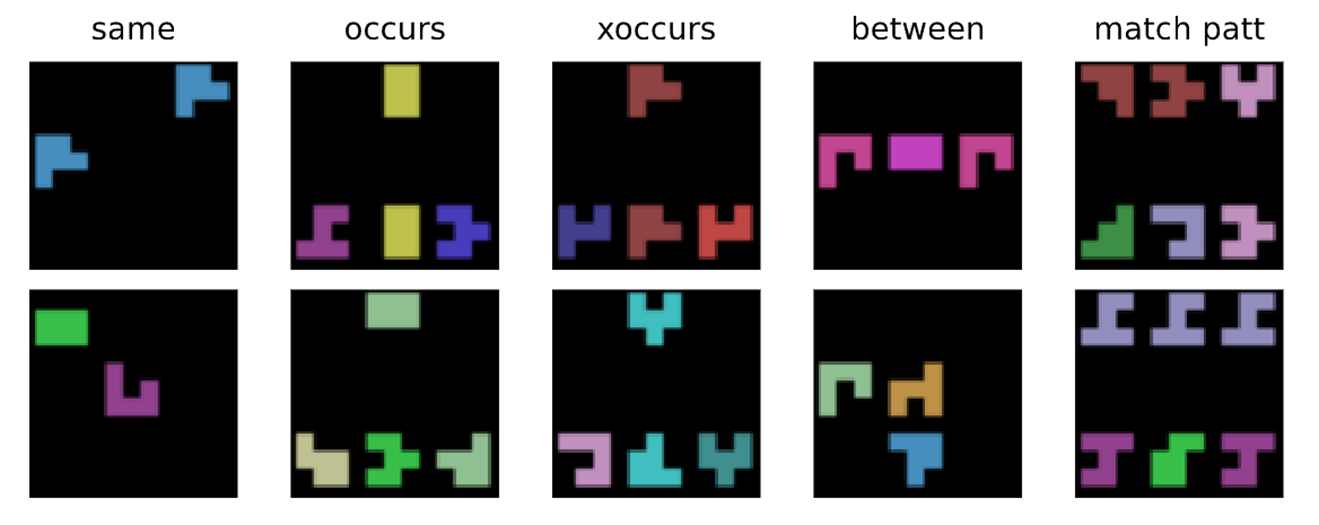
\includegraphics[width=\linewidth]{figs/relgames_example.png}
        % \caption{Relational Games tasks from Shanahan et al. (2020)}
    \end{figure}
    \begin{center}
      Relational Games tasks from Shanahan et al. (2020)
    \end{center}
    A \alert{Visual Relational Reasoning Task}: \newline
    \qquad determine whether a particular relation holds or not

\end{frame}

\begin{frame}
    Humans have a natural ability and a preference to do relational reasoning

    We enjoy it (make games out of it)

    Cab reason about relations, \alert{abstracted} away from sensory features
\end{frame}

% swap with above
\begin{frame}{Big Picture:\\Why should we care about ``relational reasoning''?}
    \begin{itemize}
        \item Cornerstone of 
        \item Point 2
        \item Point 3
    \end{itemize}
\end{frame}

\begin{frame}[standout]
    % Quote: ...
    \begin{center}
        \textit{``Quote'' --- Someone}
    \end{center}
\end{frame}

\begin{frame}[standout]
    We'd like to take a step towards this grand goal
\end{frame}

\begin{frame}
  \frametitle{Outline of Remainder of Talk}
  \begingroup
  \setbeamercolor{section in toc}{fg=gray}
  \tableofcontents[sections={1}]
  \endgroup
  \tableofcontents[sections={2-}]
\end{frame}

\section{Main Idea \& Goal}

\begin{frame}{Some Lessons from Previous Work}
    \tiny{
    Prior works on relational inductive biases
    \begin{itemize}
        \item Santoro et al. ``\textit{A simple neural network module for relational reasoning}' (2017)
        \item Shanahan et al. ``\textit{An Explicitly Relational Neural Network Architecture}'' (2020)
        \item Kerg et al. ``Inductive biases for relational tasks'' (2022)
        \item Others...
    \end{itemize}
    }
    \normalsize
    \begin{center}
        \emph{\alert{Data-efficient relational reasoning requires inductive biases}}
    \end{center}

    \begin{itemize}
        \item Standard neural models (e.g., Transformers) are \alert{\emph{data-\underline{in}efficient}} at learning relational tasks; brittle OOD generalization
        \item \alert{Basic idea:} constrain model to compute relational features (``subtractive'')
    \end{itemize}
\end{frame}

\begin{frame}{Tension: Generality vs. Inductive Biases}
    \begin{itemize}
        \item \alert{However}, these models are narrow in domain
        \item They improve relational processing, but \alert{lose generality}
        % \item Empirical success limited to synthetic benchmarks
    \end{itemize}
\end{frame}

\begin{frame}{Tension: Generality vs. ...}
    \begin{itemize}
        \item Tension between ...
        \item e.g.,
        \item Transformer architecture: a promising backbone/basis for ...
    \end{itemize}
\end{frame}

\begin{frame}{How to imbue Transformers with explicit relational inductive biases}
    \begin{itemize}
        \item \textit{Inductive Bias}: [define]
        \item \textit{Our Philosophy:} Two types
        \begin{itemize}
            \item Additive: [define] [frame slide highlight]
            \item Subtractive: [define]
        \end{itemize}
    \end{itemize}
\end{frame}

\begin{frame}[standout]
    Let's augment the Transformer architecture with explicit relational mechanisms \& inductive biases
\end{frame}

% Include "aside" on related work / literature?
\begin{frame}{The Transformer architecture, essentially}
    \begin{itemize}
        \item Iterate two basic operations:
        \begin{enumerate}
            \item Information Retrieval (Attention)
            \item Local Processing (Token-wise MLP)
        \end{enumerate}
    \end{itemize}
\end{frame}

\begin{frame}{How to imbue Transformers with explicit relational inductive biases}
    \begin{itemize}
        \item Strength of Transformers: \alert{\emph{attention}} \newline
        ``\textit{The Unreasonable effectiveness of attention}''
        \begin{itemize}
            \item Versatile information retrieval mechanism
            \item Composable in \alert{\textit{circuits}} to carry out complex computation \newline \tiny{(which we're now beginning to understand with more systematic interp work)}
        \end{itemize}
        \item
    \end{itemize}
\end{frame}

\section{The Sensory and the relational}
\begin{frame}{Two types of information}
    \begin{itemize}
        \item Fundamentally, attention is an information retrieval operation
        \item Two key \textit{types} of information
        \item Sensory: [definition / examples]
        \item Relational: [definition / examples]
    \end{itemize}
\end{frame}

\begin{frame}{Two types of attention}
    \begin{itemize}
        \item (Standard) Sensory Attention: ...
        \item Relational Attention: ... [highlight in next frame]
    \end{itemize}
\end{frame}

% \begin{frame}{Two types of attention}
%     \begin{block}{Block Title}
%         Content goes here.
%     \end{block}
% \end{frame}

\section{Relational Attention}
\begin{frame}{High-level: Relational Attention}
    % high-level : 1) attend; 2) relate; 3) tag with symbols
    {\LARGE
    \begin{enumerate}
        \item Attend
        \item Relate
        \item Tag with symbols
    \end{enumerate}
    }
\end{frame}

\begin{frame}{Attention}
    \begin{itemize}
        \item Summary of key points
        \item Final thoughts
    \end{itemize}
\end{frame}

\begin{frame}{Computing Relations}
    \begin{itemize}
        \item Summary of key points
        \item Final thoughts
    \end{itemize}
\end{frame}

\begin{frame}{Symbols (High-Level)}
    \begin{itemize}
        \item ...
    \end{itemize}
\end{frame}

\begin{frame}{Relational Attention}
    \begin{align*}
        \RelAttn(x, (\ys)) = ...
    \end{align*}
\end{frame}

\begin{frame}{A few comments...}
    \begin{itemize}
        \item ...
    \end{itemize}
\end{frame}

\section{Dual Attention Transformer Architecture}

\begin{frame}{...}
    \begin{itemize}
        \item ...
    \end{itemize}
\end{frame}

\section{Empirical Investigation}
\begin{frame}{Prelude: what questions are we trying to answer?}
    \begin{itemize}
        \item ...
    \end{itemize}
\end{frame}


\section{Concluding Remarks}

\begin{frame}{Concluding Remarks}
    \begin{itemize}
        \item ...
    \end{itemize}
\end{frame}


\begin{frame}{Thank you! Discussion Time...}
    \begin{itemize}
        \item \alert{Joint work} with \emph{John Lafferty}
        \item \alert{Supported by funding from} ARNI NSF AI Institute
        \item \alert{Paper:} \href{https://arxiv.org/abs/2405.16727}{\texttt{arXiv:2405.16727}} / ICML '25
        \item \alert{Project webpage:} {\small \url{https://awni.xyz/dual-attention/}} %\url{www.awni.xyz/dual-attention}
        \begin{itemize}
            \item Open weights on HF (DAT-LM up to 1.3B-params)
            \item Implementation available via python package\newline
            \hphantom{~~~~~} \texttt{pip install dual-attention}
        \end{itemize}
        \item \alert{Personal webpage:} {\small \url{https://awni.xyz}}
    \end{itemize}
\end{frame}

% \begin{frame}[standout]
%     \textit{Thank you!}
% \end{frame}

\end{document}